\chapter{Detectability in IM Surveys}
\label{chapter:snrska}


%
%
%---------------------------
%
%
\section{21cm intensity mapping surveys}
%
Some blah blah about intensity mapping 
%
\section{Introduction}
%

}
%
%
%---------------------------------------------
%
%
\section{Relativistic effects in the 21cm intensity bispectrum}
%

%
%-----------------------------------------------------------
%
%
\section{Relativistic signal-to-noise ratio}
%
{The signal-to-noise ratio for a bispectrum in the Gaussian case is given by 
$\mathrm{SNR}^2 = {B^2 / \mathrm{Var}(B)}$, where the variance includes cosmic variance as well as noise.
The relativistic part of the bispectrum at leading order is extracted as the imaginary part of the estimator for the bispectrum. For the variance, we use the fact that it is unaffected by relativistic corrections at leading order: $\mathrm{Var}(B_{\hi})= \mathrm{Var}(B_{\mathrm N})+O(\cH^2/k^2)$, as shown in \cite{Maartens:2019yhx}.}
%
The bispectrum in each $z$-bin has 5 independent degrees of freedom, which we choose as the 3 sides $k_a$ of the closed triangle and 2 angles $(\theta_1=\cos^{-1}\mu_1,\varphi)$
that define the orientation of the triangle.
The relativistic SNR per $z$-bin is then given by  \cite{Maartens:2019yhx}
\begin{equation}
{{\mathrm{SNR}}(z)^2 =
\sum_{k_a,\mu_1,\varphi}\,\frac{B_{\mathrm D}(z, k_{a},  \mu_{1},\varphi) \,B_{\mathrm D}^*(z, k_{a},  \mu_{1},\varphi)}{{\mathrm Var} [{B_{\mathrm N}}(z, k_a,\mu_{1},\varphi)]}\,,} \label{e2.2_0}
\end{equation}
where we isolated the imaginary part, 
and the cumulative SNR is defined by
\begin{equation}
{{\mathrm SNR}(\leq z)^2 =
\sum_{z'}\,{\mathrm SNR}(z')^2\,.} \label{csnr_d2ß}
\end{equation}
The total SNR is  $\mathrm{SNR}(\le z_\mathrm{max})$.

The variance is estimated as 
\begin{equation}
\!\!\!{\mathrm{Var} [{B_{\mathrm N}}(z, k_a,\mu_{1},\varphi)]}
=\frac{s_B\,\pi\, k_{\mathrm f}(z)^3}{k_1k_2k_3 (\Delta k)^3}\,\frac{{4\pi}}{ \Delta \mu_1 \Delta \varphi} \,
\tilde{P}_{\hi}(z,k_{1},\mu_{1})\,\tilde{P}_{\hi}(z,k_{2},\mu_{2}) \,\tilde{P}_{\hi}(z,k_{3},\mu_{3})\,.
\label{e2.7}
\end{equation}
Here
\begin{equation}
\tilde{P}_{\hi}(z, k, \mu) = P_{\hi}(z, k, \mu) + P_\mathrm{noise}(z,k,\mu)\,, \label{e2.4}
\end{equation}
where the HI power spectrum is Newtonian at leading order: $P_{\hi}= P_{\hi} +O(\cH^2/k^2)$, with
\begin{equation}
P_{\mathrm N}(z, k, \mu) = \big[b_{1}(z)+f(z)\mu^{2}\big]^{2}P_{\mathrm m}(z,k)\,.\label{e2.5_1}
\end{equation}
In \eqref{e2.7}, the multiplicity constant $s_B=6, 2, 1$ for equilateral, isosceles, and non-isosceles triangles,  and $\Delta k,\Delta \mu_1,  \Delta \varphi$ are bin widths. We follow \citep{Karagiannis:2018jdt,Maartens:2019yhx} and choose the step lengths as
\begin{equation}
\Delta z = 0.1\,, \quad \Delta \mu = 0.04\,, \quad {\Delta\varphi=\pi/25}\,, \quad \Delta k(z) = k_{\mathrm{f}}(z)\,.\label{e4.1} 
\end{equation} 
The fundamental mode $k_{\mathrm{f}}$ is an estimate of  the minimum wavenumber included in the survey, and is determined in each redshift bin  by the comoving volume of the bin centred at $z$:
\begin{equation}
k_{\mathrm{f}}(z) = \frac{2\pi}{V(z)^{1/3}} \quad \mbox{with} \quad V(z) = \frac{4\pi}{3}f_{\mathrm{sky}} \big[r(z+{\Delta z}/{2})^{3} - r(z-{\Delta z}/{2})^{3} \big] \,.\label{e2.8}
\end{equation}
Here $f_{\mathrm{sky}}=\Omega_\mathrm{sky}/4\pi$ is the sky fraction covered by the survey.
%
%
%-----------------------------------
%
%
\subsection{Nonlinearity}
%
The tree-level bispectrum is a perturbative model. In order to avoid scales where dark matter clustering becomes nonperturbative, we impose a maximum scale \cite{Maartens:2019yhx}
\begin{equation} \label{eq:snrkmax}
k_{\mathrm{max}}(z) = 0.1h\,(1+z)^{2/(2+n_s)}~\mathrm{Mpc}^{-1}\,.
\end{equation}
However, applying this cut-off still includes nonperturbative RSD effects, i.e. the fingers-of-god damping. In order to take account of this, we follow \cite{Karagiannis:2018jdt,Yankelevich:2018uaz,Maartens:2019yhx} and use the following phenomenological model of the damping of redshift-space clustering due to nonlinear velocities:
\begin{align}
 P_{\hi}(k,\mu,z) & ~\to~   \exp\Big[-\frac{1}{2}{k^2\mu^2\,{\sigma_{P}(z)}^{2}}\Big]\,P_{\hi}(k,\mu,z)
 \,, \label{e2.10}\\
 B_{\hi}(k_a,\mu_a,z) & ~\to~  \exp\Big[-\frac{1}{2}{\left( k_{1}^{2}\mu_{1}^{2}+k_{2}^{2}\mu_{2}^{2}+k_{3}^{2}\mu_{3}^{2}\right){\sigma_{B}(z)}^{2}}\Big]\,B_{\hi}(k_a,\mu_a,z)
 \,. \label{e2.11}
\end{align}
Damping is effective for $k\gtrsim \sqrt{2}/\sigma_P$ for the power spectrum and  $k\gtrsim \sqrt{2}/\sigma_B$ for the bispectrum.
In this model, the damping parameters $\sigma_P$ and $\sigma_B$ are  to be determined by data or simulations.
We use a model for the power spectrum damping parameter based on HI simulations \cite{Sarkar:2019ojl}:
\begin{equation}
\sigma_{P}(z) = 11h\big(1+z\big)^{-1.9}\exp{\big[-(z/11)^{2}\big]}~~h^{-1}\,\mathrm{Mpc}\,. \label{e2.12}  \\
\end{equation}
We are not aware of any simulation-based expression for $\sigma_B$, and we therefore take $\sigma_B=\sigma_P$ as a first approximation. The
effect of increasing $\sigma_B$ is discussed in Section ref sec5.

A further source of nonlinearity on weakly nonlinear scales that contributes to the bispectrum variance  is the non-Gaussian effect due to mode coupling. We follow \cite{Karagiannis:2018jdt,Maartens:2019yhx} and  take account of this using the simple model developed in \cite{Chan:2016ehg}, which modifies the variance as follows: 
\begin{equation}
\mathrm{Var} [{B_{\mathrm N}}(\k_a)]  \to  \mathrm{Var}  [{B_{\mathrm N}}(\k_a)] \left[1+  
\frac{\delta\tilde{P}_{\mathrm N}(\k_1)}{\tilde{P}_{\mathrm N}(\k_1)} + \frac{\delta\tilde{P}_{\mathrm N}(\k_2)}{\tilde{P}_{\mathrm N}(\k_2)} + \frac{\delta\tilde{P}_{\mathrm N}(\k_3)}{\tilde{P}_{\mathrm N}(\k_3)}\right]  .
 \label{eq:e2.14}
\end{equation}
 Here the redshift dependence  has been dropped for brevity, and
\begin{align}
\delta\tilde{P}_{\mathrm N}(\k) & = \tilde{P}_{\mathrm N}^{\nl}(\k) - \tilde{P}_{\mathrm N}(\k)\,, 
\label{eq:e2.15}\\
\tilde{P}^{\nl}_{\mathrm N}(\k) =& \big(b_{1}+f\mu^2\big)^2P^{\nl}_{\mathrm m}(k)+P_\mathrm{noise}(\k)\,,\label{e2.15_1}
\end{align}
where $\tilde{P}_{\mathrm N}={P}_{\mathrm N}+P_\mathrm{noise}$ and
$P^{\nl}_{\mathrm m}$ is the nonlinear matter power spectrum computed in CLASS with a modified Halofit emulator.
%
%
\subsection{Effects of foregrounds}
%
\subsection{Maximum and minimum scales probed}
%
\subsection{Instrumental noise}
%
\subsection{Future HI intensity mapping surveys}
%
We consider surveys proposed for the following dish arrays:
\begin{itemize}
\item 
SD mode:  MeerKAT, 
SKA1-MID.
\item
IF\ mode: HIRAX,
PUMA (Petite). 
\end{itemize}
The survey specifications are given in Table~\ref{tab:tab1}, {based on~\cite{Santos:2017qgq, Bacon:2018dui, Slosar:2019jwd,Karagiannis:2019jjx,Castorina:2020zhz}}. {Limiting wavenumbers for large wavelengths  are shown for these surveys in Figure \ref{figmin}: the
fundamental wavenumber \eqref{e2.8}, the minimum radial wavenumber \eqref{kfgpar} from foreground cleaning and the IF-mode minimum wavenumber \eqref{kifmin}.}
%\vspace{-0.5cm}

\begin{table}[ht]
\centering
\caption{\label{tab:tab1} {HI intensity mapping survey specifications. 
(For *, see Appendix REF APPENDIX 2 OF IM)}} 
\vspace*{0.2cm}
\begin{tabular}{|lccccccc|} \hline
Survey & Redshift range & $f_\mathrm{sky}$ & $t_{\mathrm{tot}}$  & $T_{\mathrm{d}}$ & $D_\mathrm{d}$ & $N_\mathrm{d}$ & {$D_\mathrm{max}$} \\
&  & & [$10^{3}$ hr] & [K]  & [m] & & {[m]} \\
\hline\hline 
MeerKAT L Band   & 0.10--0.58 & 0.10 & 4  & * & 13.5 & 64 & -- \\
MeerKAT UHF Band & 0.40--1.45 & 0.10 & 4  & * & 13.5 & 64  & --  \\
SKA1-MID Band 1  & 0.35--3.05 & 0.48 & 10 & * & 15.0 & 197  & --  \\
SKA1-MID Band 2  & 0.10--0.49 & 0.48 & 10 & * & 15.0 & 197  & --  \\
HIRAX            & 0.75--2.00 & 0.36 & 10 & 50 & 6.0  & 1024  & {270}\\
PUMA (Petite)    & 2.00--6.00 & 0.50 & 40 & 50 & 6.0  & 5000 & {600} \\
\hline
\end{tabular}
\end{table}

\vspace*{-0.5cm}
\begin{table}[ht]
\centering
\caption{\label{tab2} {Parameters in \eqref{e3.4}} (from~\cite{Ansari:2018ury}).} 
\vspace*{0.2cm}
\begin{tabular}{|lcccccl|} \hline
Survey & $a$ & $b$ & $c$  & $d$ & $e$ & $N_\mathrm{s}$  \\ \hline\hline 
HIRAX & 0.4847 & $-0.3300$ & 1.3157 & 1.5974 & 6.8390 & 32  \\
PUMA (Petite) & 0.5698 & $-0.5274$ & 0.8358 & 1.6635 & 7.3177 & {100} \\
\hline
\end{tabular}
\end{table}

For the system temperature, we use the results of measurements and simulations for MeerKAT and SKA1-MID, given in Appendix REF APP IM. For HIRAX and PUMA, we use the fit \eqref{e2.25}. 


In IF mode, HIRAX is assumed to be a square-packed array, while PUMA is taken as hexagonal-packed in a circular area, {with 50\% fill factor}. We follow~\cite{Karagiannis:2019jjx} and use the fitting formula from~\cite{Ansari:2018ury} for the baseline density of such arrays:
\begin{equation}
n_\mathrm{b}^\mathrm{phys}(L) = \left( \frac{N_\mathrm{s}}{D_\mathrm{d}}\right)^2\,\frac{a+b\big(L/L_\mathrm{s}\big)}{1+c\big(L/L_\mathrm{s}\big)^{d}}\,\exp{\big[-(L/L_\mathrm{s})^{e}\big]}\,, \label{e3.4}
\end{equation}
where  $L_\mathrm{s} =N_\mathrm{s}D_\mathrm{d}$ and $N_\mathrm{s}^2 = N_\mathrm{d}$.
The  parameters in \eqref{e3.4} are given in Table \ref{tab2}, {and $n_\mathrm{b}^\mathrm{phys}(L)$ is shown in Figure~\ref{nbphys}.
\begin{figure}%[h]
%\vspace*{-0.5cm}
\centering
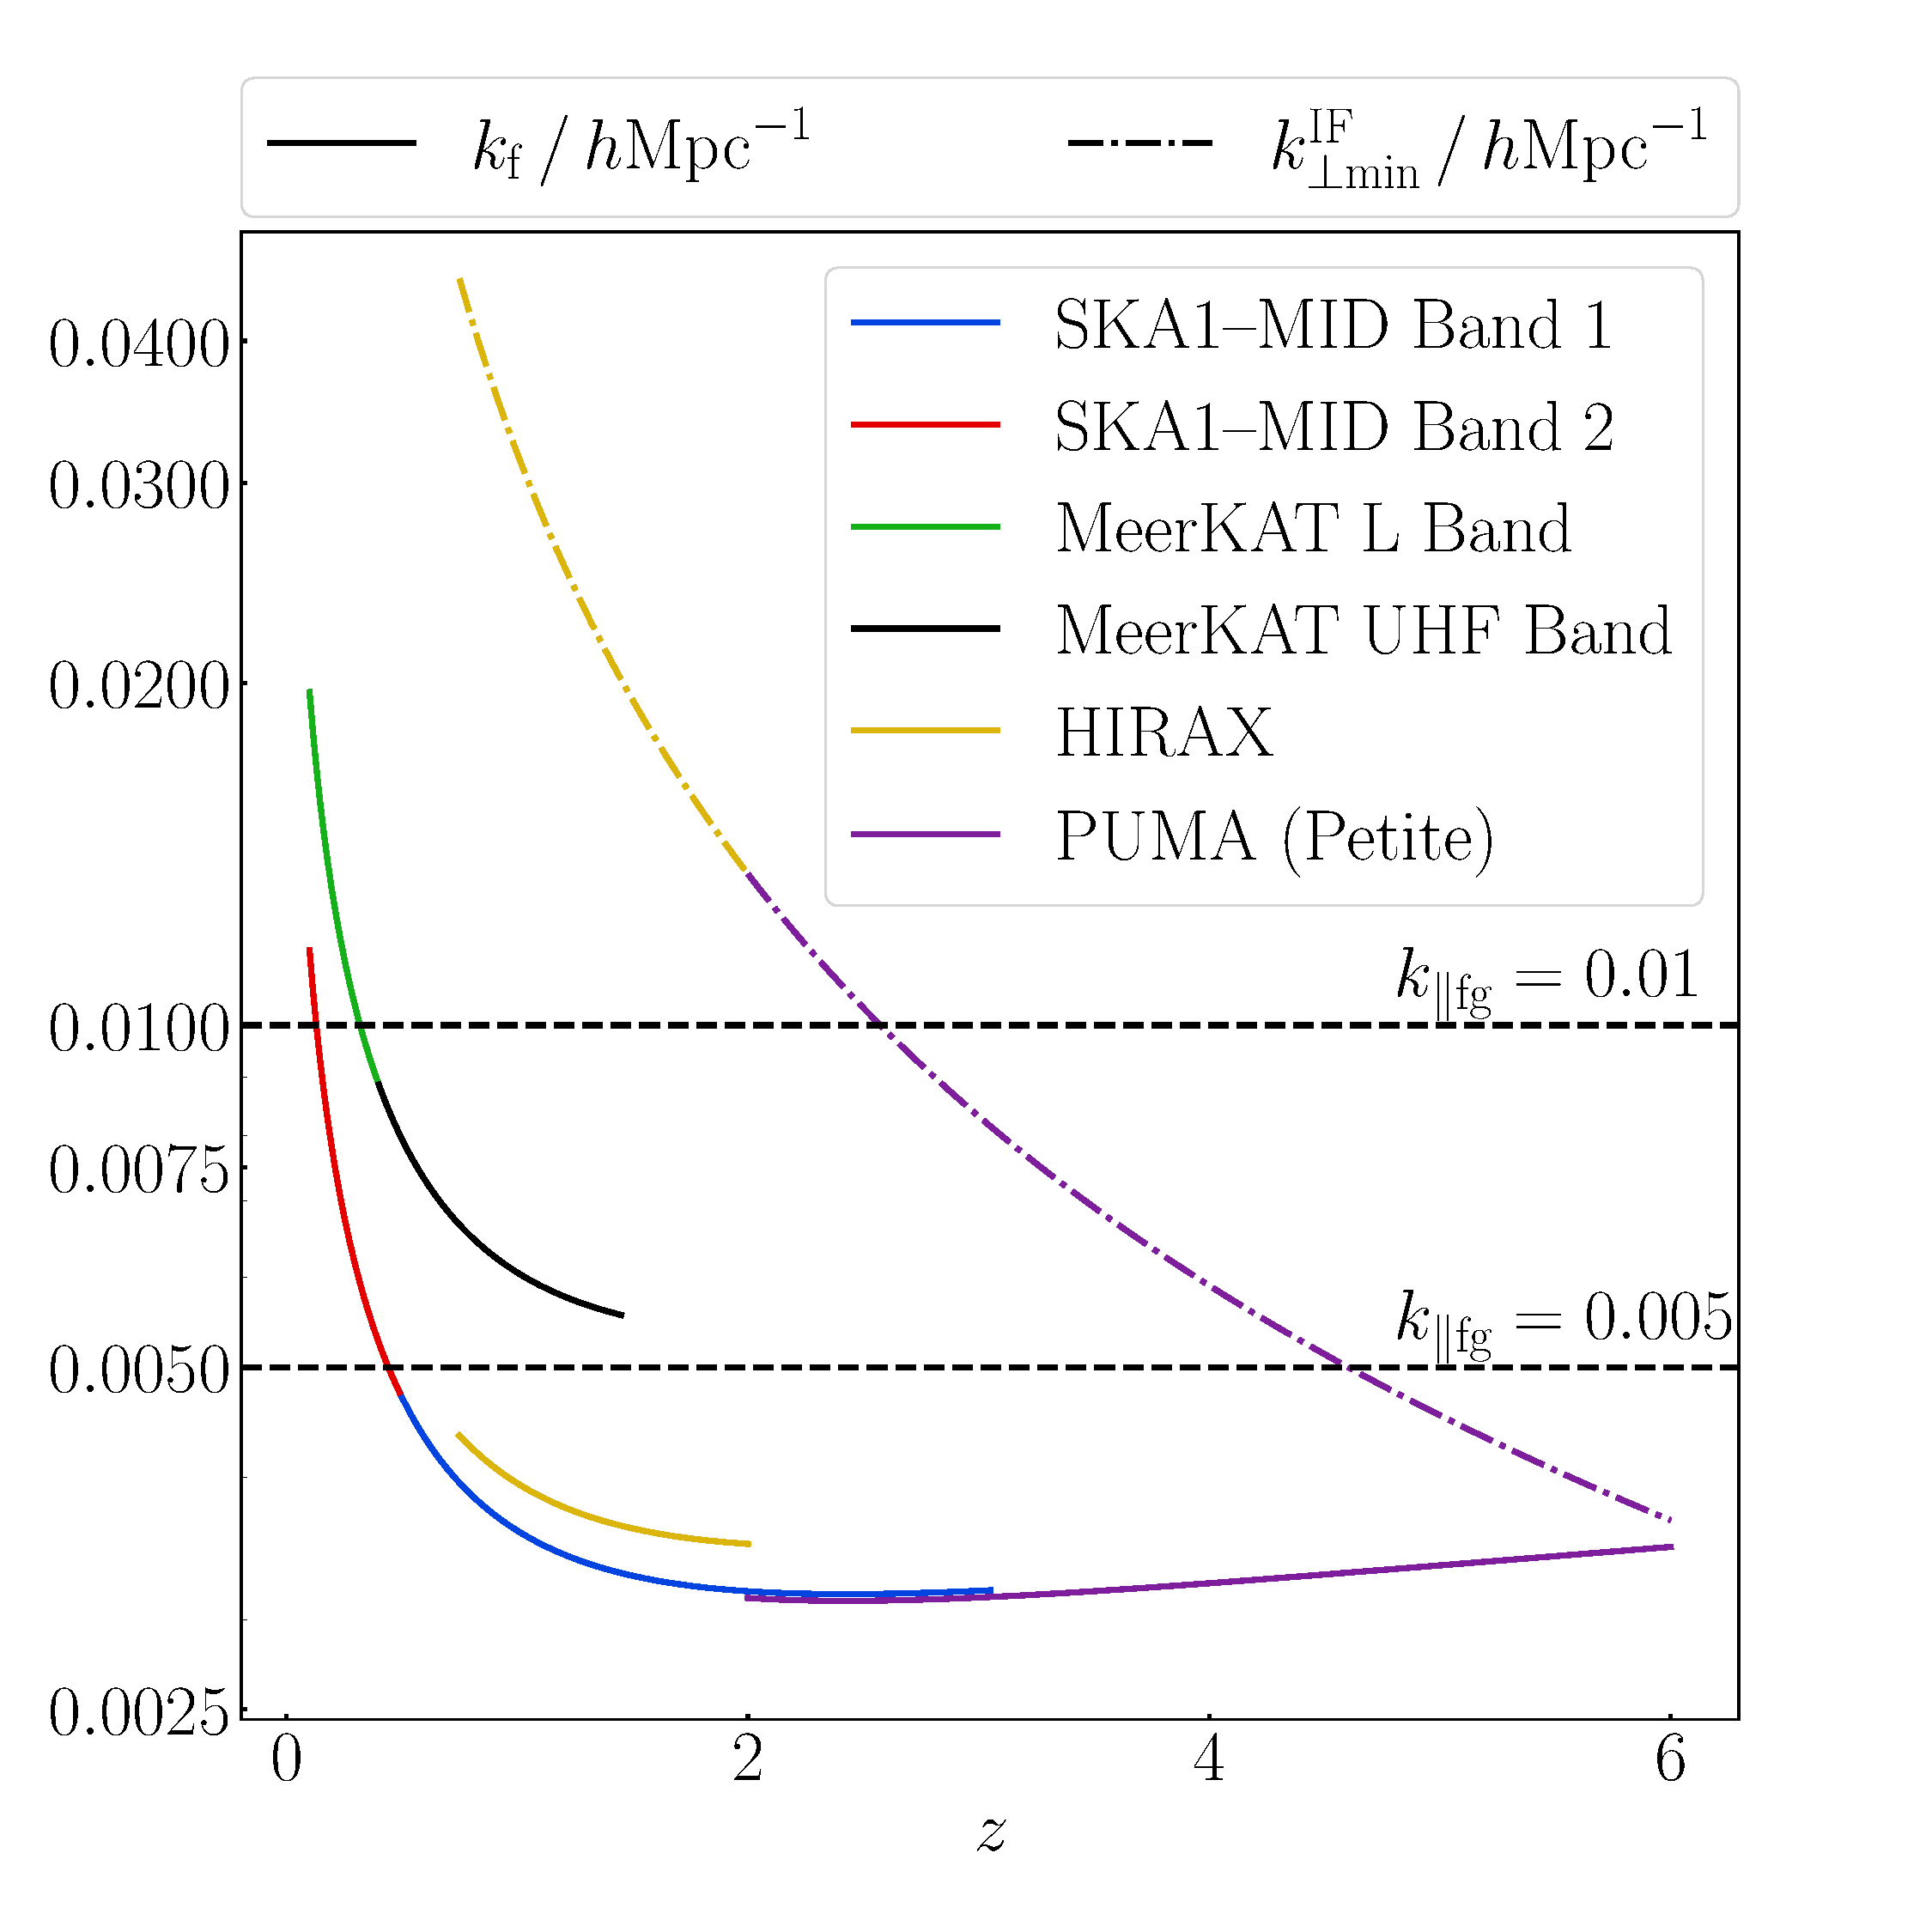
\includegraphics[width=.49\textwidth]{fig/k}
%\vspace*{-0.5cm}
\caption{{Minimum wavenumbers for the surveys, where $k$ is subject to \eqref{kmin} (SD) or \eqref{kminif} (IF).}}\label{figmin}
\end{figure}

%\vspace*{-0.5cm}
\begin{figure}[ht]
\centering
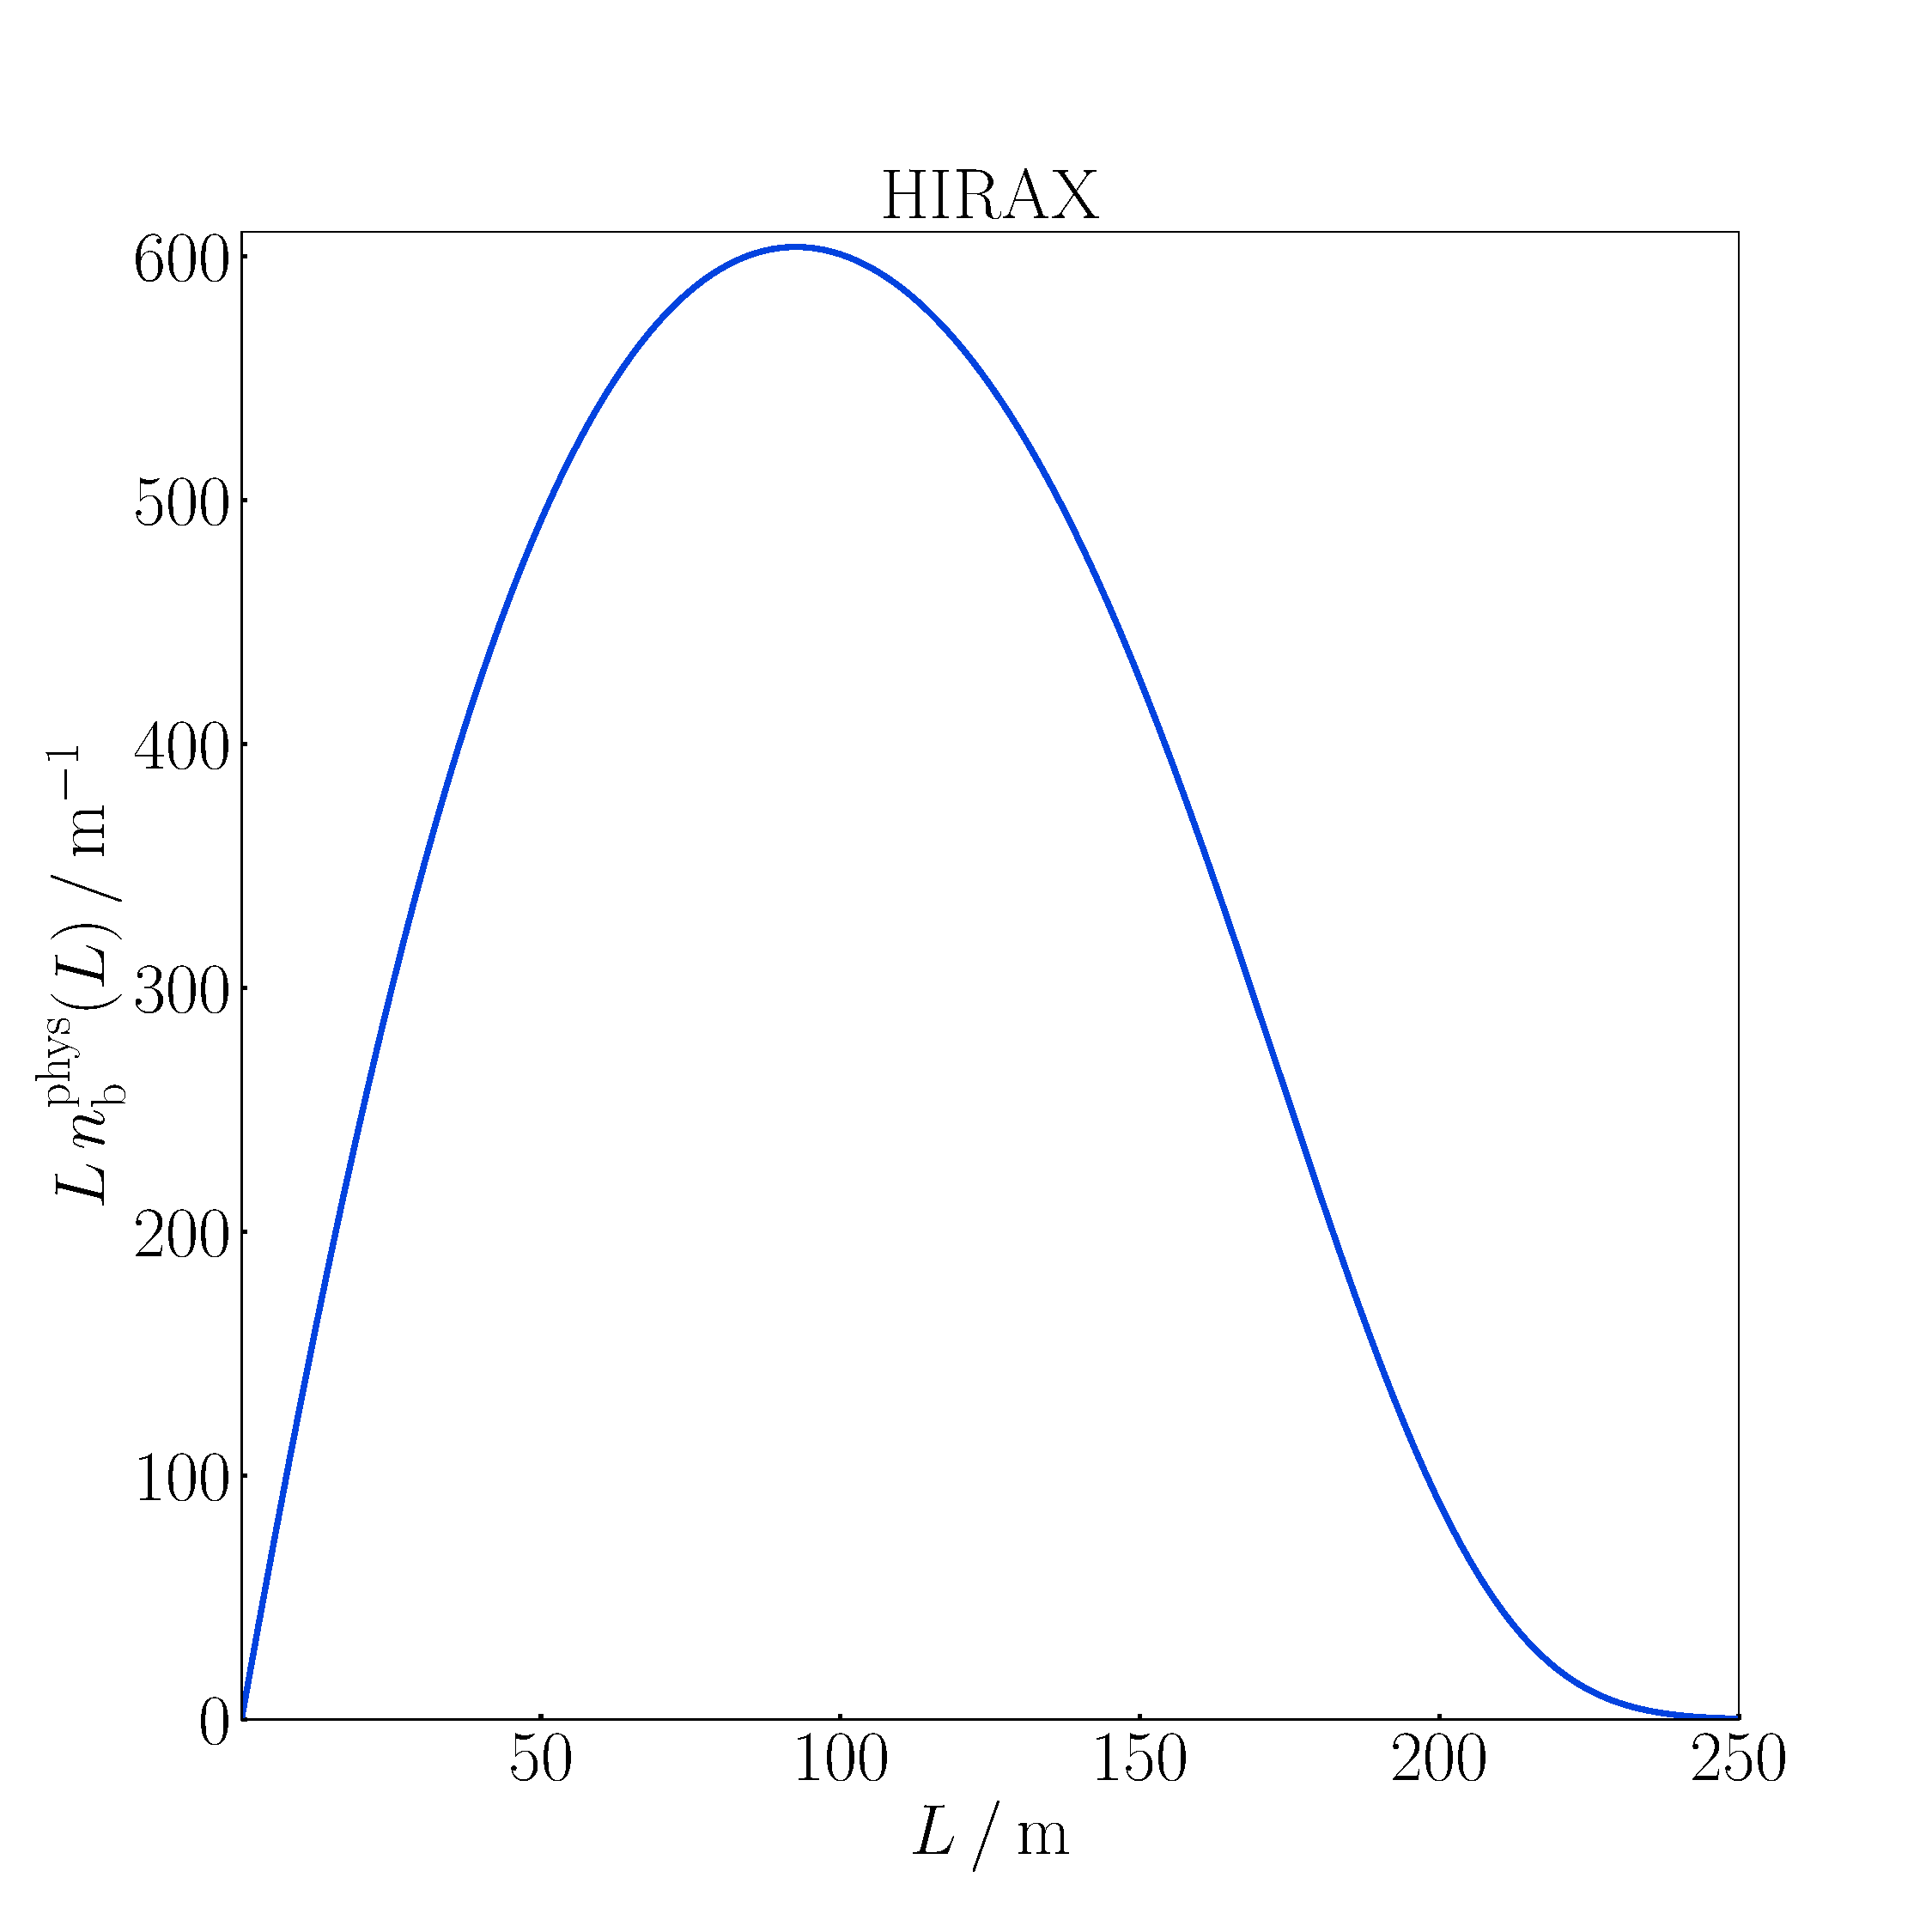
\includegraphics[width=.49\textwidth]{fig/nbHIRAX}
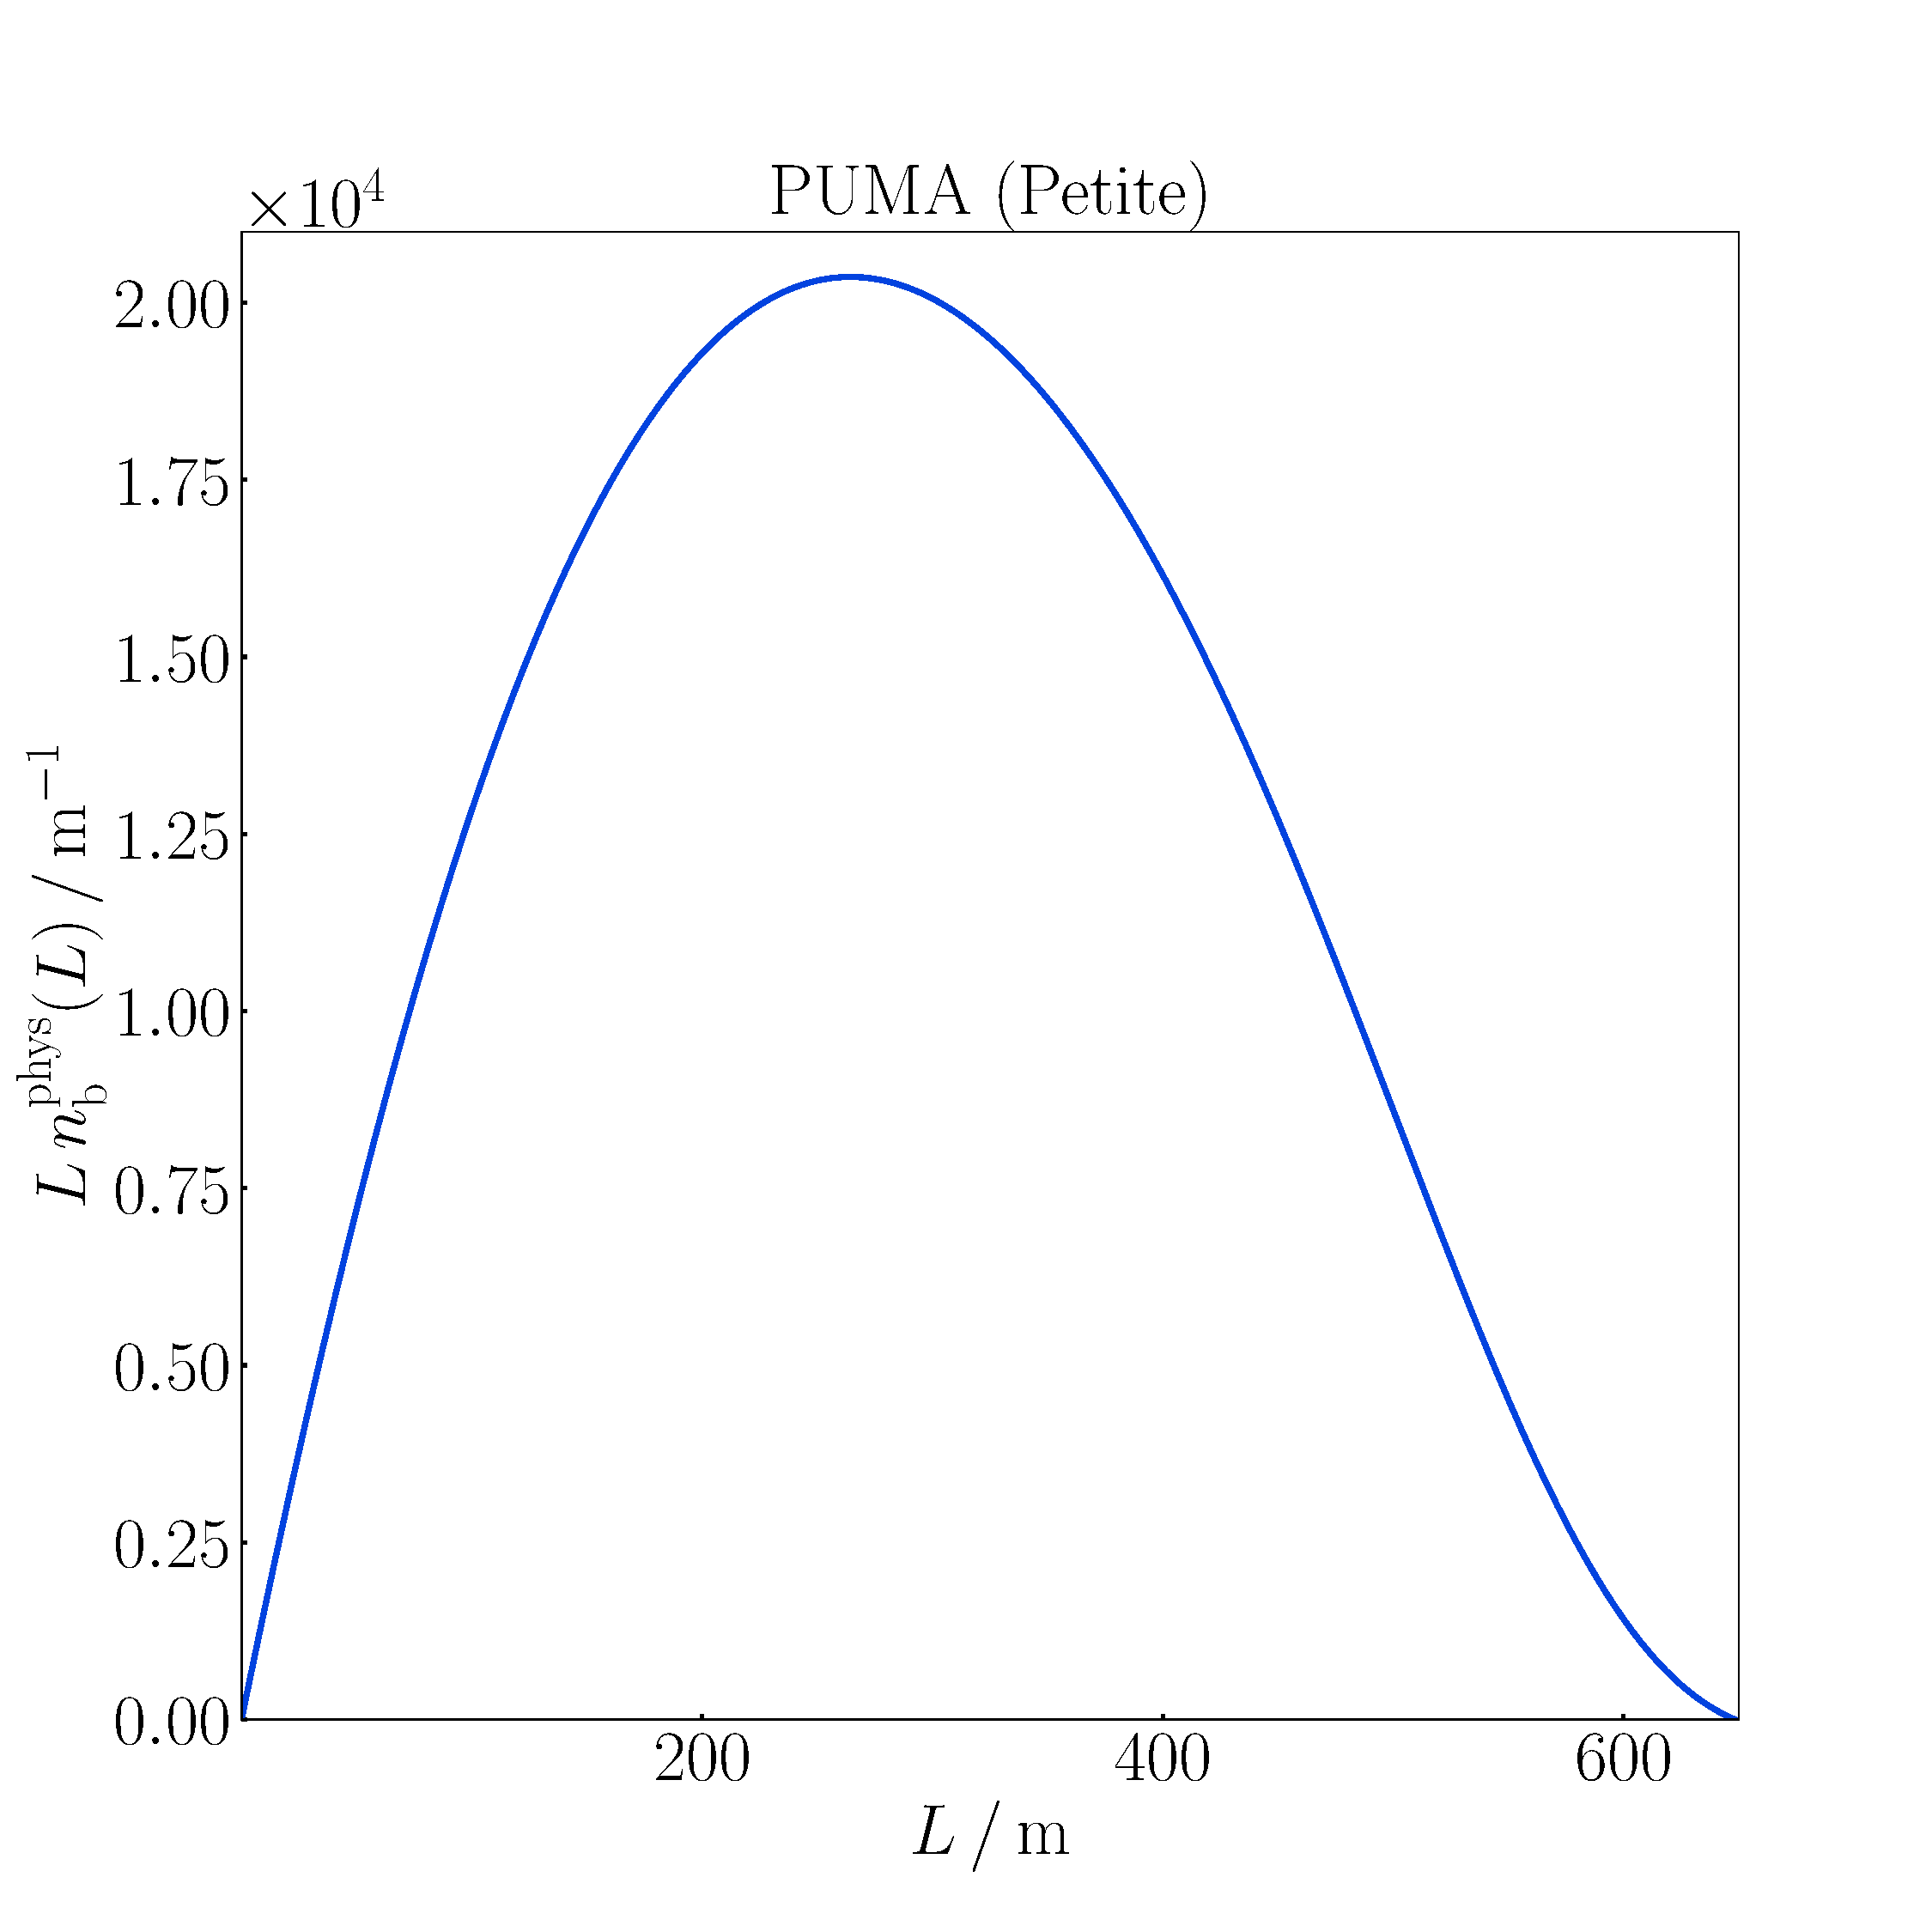
\includegraphics[width=.49\textwidth]{fig/nbPUMAPetite}
\vspace*{-0.5cm}
\caption{Physical baseline density models for HIRAX (left) and PUMA (right).}\label{nbphys}
\end{figure}
%\vspace*{-0.5cm}
\begin{figure}[!ht]
\centering
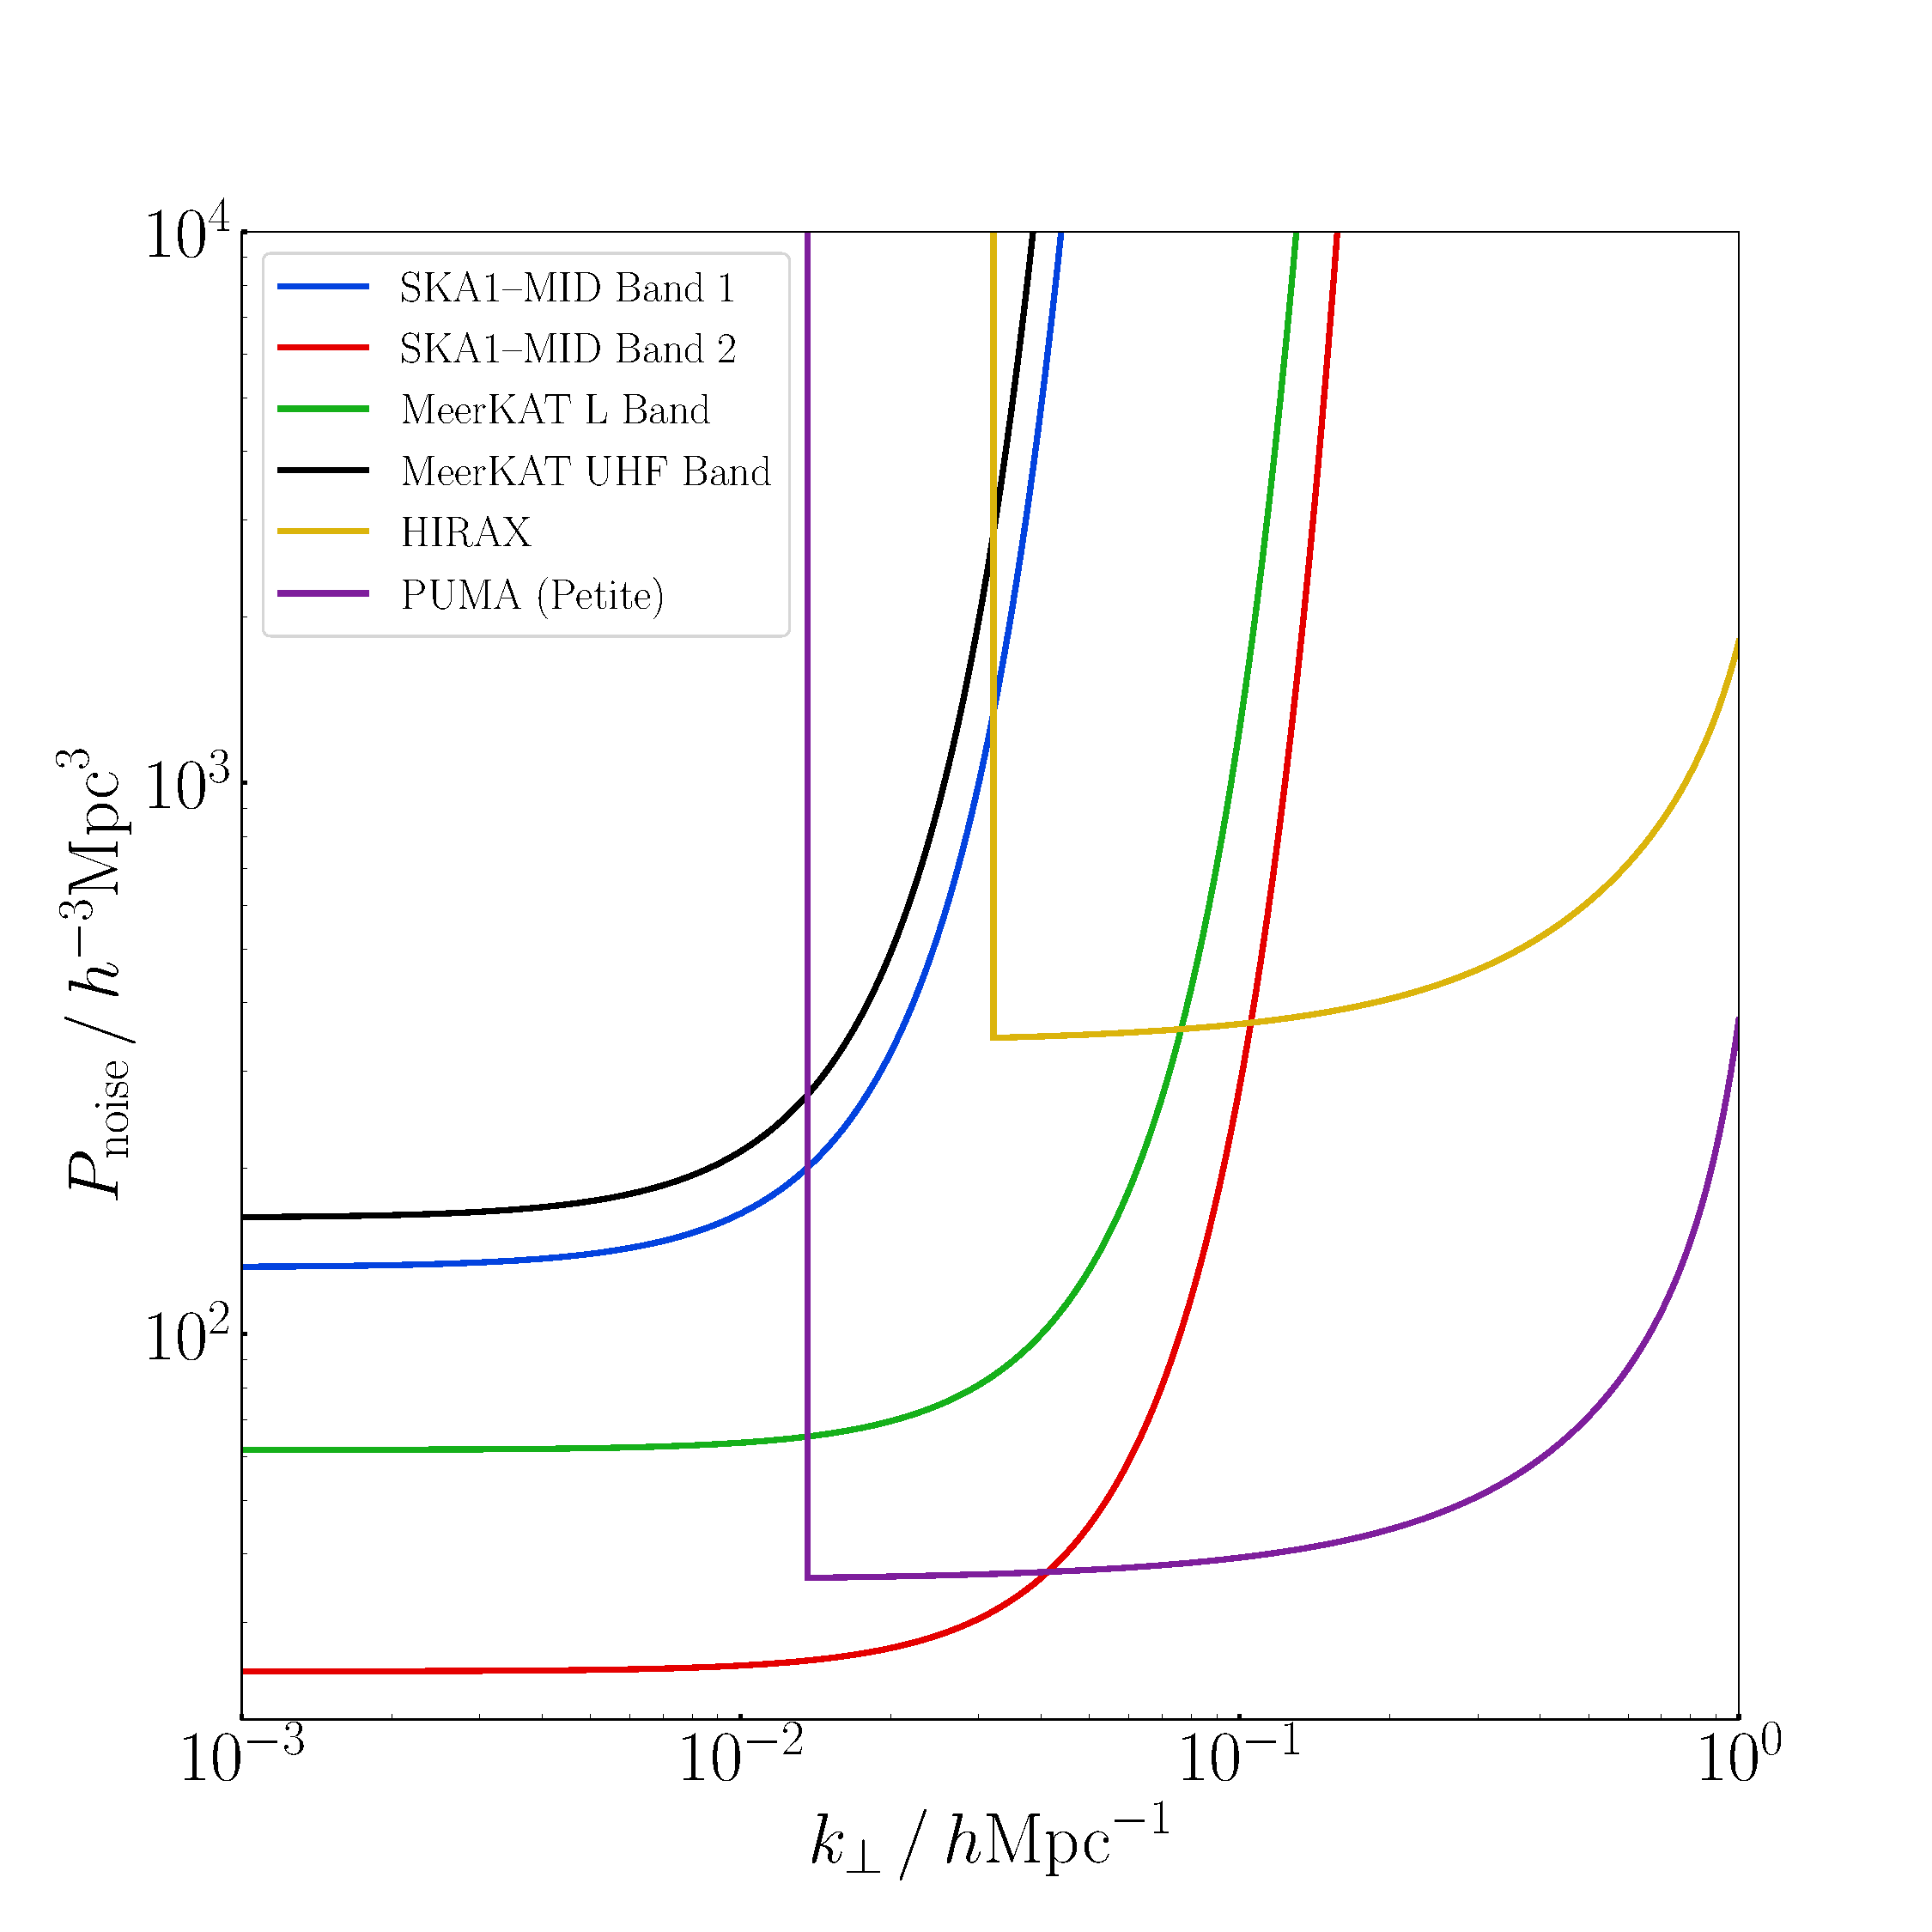
\includegraphics[width=.49\textwidth]{fig/Pnoise}
\vspace*{-0.5cm}
\caption{{Noise power spectra of the SD-mode surveys (at $z=0.4$ for low-$z_\mathrm{max}$ bands and $z=1$ for high-$z_\mathrm{max}$ bands) and IF-mode surveys (HIRAX at $z=1$, PUMA at $z=2$).}}\label{pnoise}
\end{figure}

{In the case of PUMA, we take account of the 50\% fill factor as follows. We use double the number of dishes to define $N_\mathrm{s}$ for the computation of \eqref{e3.4}, i.e. $N_\mathrm{s}^2= 2\times 5000$. Then  we  remove half of the dishes without changing the baseline, i.e. without changing the shape and ground-area of the array.

The noise power spectra of the surveys at fixed redshift are displayed in Figure \ref{pnoise}. For SD-mode surveys, the poor angular resolution is reflected in the blow-up of noise due to the beam in \eqref{sdn}.
The minimum transverse scale for IF-mode surveys  is shown as a sharp cut-off, as in  \eqref{kifmin}, with effectively infinite noise.
 Figure \ref{pnoise} also shows the smooth blow-up of IF-mode noise on small transverse scales, which results  from the fact that 
$n_\mathrm{b}\to 0$ as the baseline approaches its maximum $D_\mathrm{max}$ (see Figure \ref{nbphys}). The unbounded increase of noise kills the signal, corresponding to the approximate cut-off scale \eqref{kifmax}.}

























